\chapter{Bayesian Methods}\label{uq:bayes}


This chapter covers specialized approaches for accelerating the Markov
chain Monte Carlo (MCMC) sampling process used within Bayesian inference.

\section{Fundamentals} \label{uq:bayes:basic}

Bayes Theorem~\cite{Jaynes}, shown in Eq.~\ref{eq:BayesThm}, is used
for performing inference.  In particular, we derive the plausible
parameter values based on the prior probability density and the data
$\boldsymbol{d}$. A typical case involves the use of a conservative prior notion of
an uncertainty, which is then constrained to be consistent with the
observational data.  The result is the posterior parameter density of
the parameters $f_{\boldsymbol{\Theta |D}}\left( \boldsymbol{\theta |d} \right)$.
\begin{equation}
{f_{\boldsymbol{\Theta |D}}}\left( \boldsymbol{\theta |d} \right) = \frac{{{f_{\boldsymbol{\Theta}}}\left( \boldsymbol{\theta}  \right)\mathcal{L}\left( \boldsymbol{\theta;d} \right)}}{{{f_{\boldsymbol{D}}}\left( \boldsymbol{d} \right)}} \label{eq:BayesThm}
\end{equation}

The likelihood function is used to describe how well a model's
predictions are supported by the data.  
%The likelihood function can be written generally as:
%\begin{equation*}
%  \mathcal{L}\left( {\theta ;d} \right) = f\left( {q\left( \theta  \right) - d} \right)
%\end{equation*}
The specific likelihood function currently used in Dakota is a Gaussian
likelihood. This means that we assume the difference between the model quantity of interest
(e.g. result from a computer simulation) and the experimental observations are Gaussian:
\begin{equation}
d_i = q_i(\boldsymbol{\theta}) + \epsilon_i, \label{eq:model}
\end{equation}
where $\boldsymbol{\theta}$ are the parameters of a model quantity of interest $q_i$ and
$\epsilon_i$ is a random variable that can encompass both measurement
errors on $d_i$ and modeling errors associated with the simulation quantity of interest 
$q_i(\boldsymbol{\theta})$. %We further assume that all experiments and
%observations are independent.  
If we have $n$ observations, the probabilistic model defined by 
Eq.~(\ref{eq:model}) results in a likelihood function for $\boldsymbol{\theta}$ 
%that is the product of $n$ normal probability density functions 
as shown in Eq.~\ref{eq:Likelihood}:
\begin{equation}
\mathcal{L}(\boldsymbol{\theta;d}) = 
\frac{1}{\sqrt{(2\pi)^n |\boldsymbol{\Sigma_d}|}}
\exp \left(
-\frac{1}{2} \boldsymbol{r}^T \boldsymbol{\Sigma_d}^{-1} \boldsymbol{r} 
\right), \label{eq:Likelihood}
%\mathcal{L}({\theta};d) = \prod_{i=1}^n \frac{1}{\sigma \sqrt{2\pi}} \exp
%\left[ - \frac{\left(d_i-\mathcal{M}({\theta})\right)^2}{2\sigma^2} \right]
\end{equation}
where the residual vector $\boldsymbol{r}$ is defined from the
differences between the model predictions and the corresponding
observational data (i.e., $r_i = q_i(\boldsymbol{\theta}) - d_i$ for $i = 1,\dots,n$),
$\boldsymbol{\Sigma_d}$ is the covariance matrix of the Gaussian data
uncertainties. %, and we omit the leading multivariate normal (MVN)
%constant $1/\sqrt{(2\pi)^n |\boldsymbol{\Sigma_d}|}$ for 
%simplicity. \footnote{In practice, omitting this MVN constant can avoid 
  %precision loss due to subtractive cancellation in log-likelihood 
  %calculations; further, this shortcut will be canceled out by the 
  %normalization factor in the denominator of Eq.~\ref{eq:BayesThm}.}. 

The negative log-likelihood is comprised of the misfit function:
\begin{equation}
M(\boldsymbol{\theta;d}) = \frac{1}{2} \boldsymbol{r}^T \boldsymbol{\Sigma_d}^{-1} 
\boldsymbol{r} % + C
\label{eq:misfit}
\end{equation}
plus contributions from the leading normalization factor 
($\frac{n}{2}\log(2\pi)$ and $\log(|\boldsymbol{\Sigma_d}|)/2$).
It is evident that dropping $\boldsymbol{\Sigma_d}$ from Eq.~\ref{eq:misfit} 
(or equivalently, taking it to be the identity) results in
the ordinary least squares (OLS) approach commonly used in
deterministic calibration.  For a fixed $\boldsymbol{\Sigma_d}$, minimizing the misfit 
function is equivalent to maximizing the likelihood function and results 
in a solution known as the maximum likelihood estimate (MLE), which will 
be the same as the OLS estimate when the residuals have no relative
weighting (any multiple of identity in the data covariance matrix).

When incorporating the prior density, the maximum {\it a posteriori}
probability (MAP) point is the solution that maximizes the posterior
probability in Eq.~\ref{eq:BayesThm}.  This point will differ
from the MLE for cases of non-uniform prior probability.

%\begin{equation}
%p(\mathbf{d}|\xi) \;=\; \text{exp}\left[-\frac{1}{2}(f(\xi)-\mathbf{d})^T\boldsymbol{\Sigma_d}^{-1}(f(\xi)-\mathbf{d})\right]
%\end{equation}
%\begin{equation}
%-\text{log}\left[p(\mathbf{d}|\xi)\right] \;=\; \frac{1}{2}(f(\xi)-\mathbf{d})^T\boldsymbol{\Sigma_d}^{-1}(f(\xi)-\mathbf{d}) \;=\; M(\xi)
%\end{equation}

\section{Proposal Densities} \label{uq:bayes:prop}

When derivatives of $q(\theta)$ are readily available (e.g.,
from adjoint-capable simulations or from emulator models such as
polynomial chaos, stochastic collocation, or Gaussian processes), we
can form derivatives of the misfit function as
\begin{eqnarray}
\nabla_{\boldsymbol{\theta}} M(\boldsymbol{\theta}) &=& \nabla_{\boldsymbol{\theta}} \boldsymbol{q}(\boldsymbol{\theta})^T\,\boldsymbol{\Sigma_d}^{-1}\,\boldsymbol{r} \label{eq:grad_misfit} \\
\nabla^2_{\boldsymbol{\theta}} M(\boldsymbol{\theta}) &=& \nabla_{\boldsymbol{\theta}} \boldsymbol{q}(\boldsymbol{\theta})^T\,\boldsymbol{\Sigma_d}^{-1}\,\nabla_{\boldsymbol{\theta}} \boldsymbol{q}(\boldsymbol{\theta}) + \nabla^2_{\boldsymbol{\theta}} \boldsymbol{q}(\boldsymbol{\theta}) \cdot \left[\boldsymbol{\Sigma_d}^{-1}\,\boldsymbol{r}\right] \label{eq:hess_misfit}
\end{eqnarray}
Neglecting the second term in Eq.~\ref{eq:hess_misfit} (a
three-dimensional Hessian tensor dotted with the residual vector)
results in the Gauss-Newton approximation to the misfit Hessian:
\begin{equation}
\nabla^2_{\boldsymbol{\theta}} M(\boldsymbol{\theta}) \approx \nabla_{\boldsymbol{\theta}} \boldsymbol{q}(\boldsymbol{\theta})^T\,\boldsymbol{\Sigma_d}^{-1}\,\nabla_{\boldsymbol{\theta}} \boldsymbol{q}(\boldsymbol{\theta}) \label{eq:hess_misfit_gn}
\end{equation}
This approximation requires only gradients of the residuals, enabling
its use in cases where models or model emulators only provide
first-order derivative information.  Since the second term in
Eq.~\ref{eq:hess_misfit} includes the residual vector, it becomes less
important as the residuals are driven toward zero.  This makes the
Gauss-Newton approximation a good approximation for solutions with
small residuals.  It also has the feature of being at least positive
semi-definite, whereas the full misfit Hessian may be indefinite in general.

%To form the MVN proposal density for the MCMC process, we define the
%proposal covariance to be the inverse of the misfit Hessian.  Since
%the full Hessian may be indefinite while the Gauss-Newton
%approximation is at least positive semi-definite, we may first attempt
%to invert the full Hessian, followed by recourse when necessary to
%inverting the Gauss-Newton approximate Hessian.

We are interested in preconditioning the MCMC sampling using an
accurate local representation of the curvature of the posterior
distribution, so we will define the MCMC proposal covariance to be the
inverse of the Hessian of the negative log posterior.  From
Eq.~\ref{eq:BayesThm} and simplifying notation to $\pi_{\rm post}$ for
the posterior and $\pi_0$ for the prior, we have
\begin{equation}
\nabla^2_{\boldsymbol{\theta}} 
  \left[ -\log(\pi_{\rm post}(\boldsymbol{\theta})) \right] = 
  \nabla^2_{\boldsymbol{\theta}} M(\boldsymbol{\theta}) - 
  \nabla^2_{\boldsymbol{\theta}} \left[ \log(\pi_0(\boldsymbol{\theta})) \right] 
\label{eq:hess_post}
\end{equation}

A typical approach for defining a proposal density is to utilize a
multivariate normal (MVN) distribution with mean centered at the current
point in the chain and prescribed covariance.  Thus, in the specific case
of an MVN proposal, we will utilize the fact that the Hessian of the
negative log prior for a normal prior distribution is just the inverse 
covariance:
\begin{equation}
-\nabla^2_{\boldsymbol{\theta}} \left[ \log(\pi_0(\boldsymbol{\theta})) \right] 
= \boldsymbol{\Sigma_0}^{-1} 
\label{eq:normal_prior_hess}
\end{equation}
For non-normal prior distributions, this is not true and, in the case
of uniform or exponential priors, the Hessian of the negative log
prior is in fact zero.  However, as justified by the approximation of
an MVN proposal distribution and the desire to improve the
conditioning of the resulting Hessian, we will employ the prior
covariance for all prior distribution types.

From here, we follow~\cite{Petra2014} and decompose the prior covariance 
into its Cholesky factors, resulting in
\begin{eqnarray}
\boldsymbol{H_{\rm nlpost}} &=& \boldsymbol{H_M} + \boldsymbol{\Sigma_0}^{-1} \\
  &=& \boldsymbol{H_M} + \boldsymbol{L}^{-T}\boldsymbol{L}^{-1} \\
  &=& \boldsymbol{L}^{-T} \left[\boldsymbol{L}^T \boldsymbol{H_M} \boldsymbol{L}
    + \boldsymbol{I} \right] \boldsymbol{L}^{-1}
\end{eqnarray}
where we again simplify notation to represent $\nabla^2_{\boldsymbol{\theta}} 
  \left[ -\log(\pi_{\rm post}(\boldsymbol{\theta})) \right]$ as 
$\boldsymbol{H_{\rm nlpost}}$ and 
$\nabla^2_{\boldsymbol{\theta}} M(\boldsymbol{\theta})$ as $\boldsymbol{H_M}$.  
The inverse of this matrix is then
\begin{equation}
\boldsymbol{H_{\rm nlpost}}^{-1} = 
  \boldsymbol{L} \left[\boldsymbol{L}^T \boldsymbol{H_M} \boldsymbol{L} +
  \boldsymbol{I} \right]^{-1} \boldsymbol{L}^T
\label{eq:inv_hess_nlpost}
\end{equation}
To address the indefiniteness of $\boldsymbol{H_M}$ (or to reduce the
cost for large-scale problems by using a low-rank Hessian approximation), 
we perform a symmetric eigenvalue decomposition of this prior-preconditioned
misfit and truncate any eigenvalues below a prescribed tolerance, resulting in
\begin{equation}
\boldsymbol{L}^T \boldsymbol{H_M} \boldsymbol{L} \approx
\boldsymbol{V}_r \boldsymbol{\Lambda}_r \boldsymbol{V}_r^T.
\end{equation}
for a matrix $\boldsymbol{V}_r$ of truncated eigenvectors and a diagonal 
matrix of truncated eigenvalues 
$\boldsymbol{\Lambda}_r = {\rm diag}(\lambda_1, \lambda_2, \dots, \lambda_r)$.
We then apply the Sherman-Morrison-Woodbury formula to invert the sum of
the decomposed matrix and identity as
\begin{equation}
\left[\boldsymbol{V}_r \boldsymbol{\Lambda}_r \boldsymbol{V}_r^T +
  \boldsymbol{I} \right]^{-1} = \boldsymbol{I} - 
  \boldsymbol{V}_r \boldsymbol{D}_r \boldsymbol{V}_r^T.
\end{equation}
for $\boldsymbol{D}_r = {\rm diag}(\frac{\lambda_1}{\lambda_1+1}, \frac{\lambda_2}{\lambda_2+1}, \dots, \frac{\lambda_r}{\lambda_r+1})$.  We now arrive
at our final result for the covariance of the MVN proposal density:
\begin{equation}
\boldsymbol{\Sigma_{MVN}} = \boldsymbol{H_{\rm nlpost}}^{-1} \approx
  \boldsymbol{L} \left[ \boldsymbol{I} - 
  \boldsymbol{V}_r \boldsymbol{D}_r \boldsymbol{V}_r^T \right] \boldsymbol{L}^T
\label{eq:inv_hess_nlpost_approx}
\end{equation}


\section{Pre-solve for MAP point} \label{uq:bayes:map}

When an emulator model is in use, it is inexpensive to pre-solve for
the MAP point by finding the optimal values for $\boldsymbol{\theta}$
that maximize the negative log posterior.  This effectively eliminates
the burn-in procedure for an MCMC chain where some initial portion of
the Markov chain is discarded, as the MCMC chain can instead be
initiated from a high probability starting point: the MAP solution.
Further, a full Newton optimization solver can be used with the
Hessian defined from Eq.~\ref{eq:hess_post}, irregardless of whether
the misfit Hessian is a full Hessian (residual values, gradients, and
Hessians are available for Eq~\ref{eq:hess_misfit}) or a Gauss-Newton
Hessian (residual gradients are available for
Eq~\ref{eq:hess_misfit_gn}).  Note that, in this case, there is no MVN
approximation as in \S\ref{uq:bayes:prop}, so we will not employ
Eq.~\ref{eq:normal_prior_hess}.  Rather, we employ the actual Hessians
corresponding to the prior distributions in use.


\section{Rosenbrock Example} \label{uq:bayes:ex}

Defining two residuals as:
\begin{eqnarray}
r_1 &=& 10 (\theta_2 - \theta_1^2) \label{eq:rosen_r1} \\
r_2 &=& 1 - \theta_1 \label{eq:rosen_r2}
\end{eqnarray}
with $\boldsymbol{d} = \boldsymbol{0}$ and $\boldsymbol{\Sigma_d} =
\text{diag}(\boldsymbol{.5})$, it is evident from Eq.~\ref{eq:misfit}
that $M(\theta;d)$ is exactly the Rosenbrock function\footnote{The
  two-dimensional Rosenbrock test function is defined as $100 (x_2 -
  x_1^2)^2 + (1 - x_1)^2$} with its well-known banana-shaped contours.

Assuming a uniform prior on $[-2,2]$,
Figure~\ref{fig:rosen_prop_covar} shows the effect of different
proposal covariance components, with the default prior covariance 
($\boldsymbol{\Sigma_{MVN}} = \boldsymbol{\Sigma_0}$) in
Figure~\ref{fig:rosen_prop_covar}(a) and a misfit Hessian-based
proposal covariance ($\boldsymbol{\Sigma_{MVN}} = \boldsymbol{H_M}^{-1}$) 
in Figure~\ref{fig:rosen_prop_covar}(b).
\begin{figure}[htbp]
  \begin{subfigmatrix}{2}
  \subfigure[Proposal covariance defined from uniform prior.]{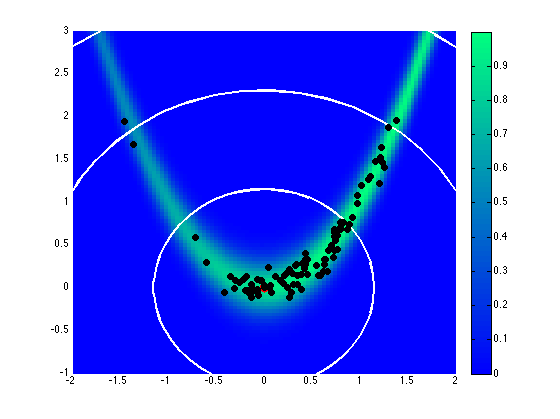
\includegraphics{images/rosen_00_prior}}
  \subfigure[Proposal covariance defined from misfit Hessian.]{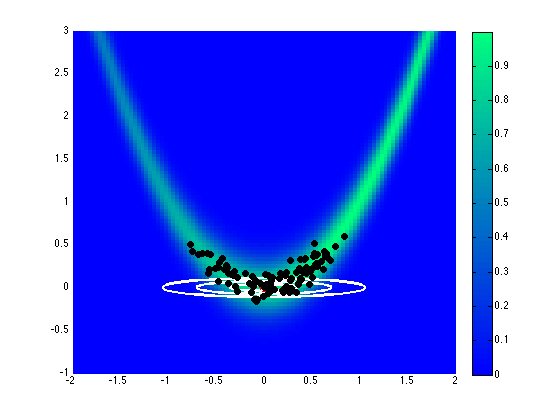
\includegraphics{images/rosen_00_pce_hessian}}
  \end{subfigmatrix}
  \caption{Depiction of proposal covariance at (0,0) with contours at one/two/three standard deviations.  2000 MCMC samples are performed and every 20th sample is plotted.}
\label{fig:rosen_prop_covar}
\end{figure}
Rejection rates for 2000 MCMC samples were 73.4\% for the former and
25.6\% for the latter.  Reducing the number of MCMC samples to 40, for
purposes of assessing local proposal accuracy, results in a similar
72.5\% rejection rate for prior-based proposal covariance and a
reduced 17.5\% rate for misfit Hessian-based proposal covariance.  The
prior-based proposal covariance only provides a global scaling and
omits information on the structure of the likelihood; as a result, the
rejection rates are relatively high for this problem and are not a
strong function of location or chain length.  The misfit Hessian-based
proposal covariance, on the other hand, provides accurate local
information on the structure of the likelihood, resulting in low
rejection rates for samples in the vicinity of this Hessian update.
Once the chain moves away from this vicinity, however, the misfit
Hessian-based approach may become inaccurate and actually impede
progress. This implies the need to regularly update a Hessian-based
proposal covariance to sustain these MCMC improvements.

In Figure~\ref{fig:rosen_restart}, we show a result for a total of
2000 MCMC samples initiated from $(-1,1)$, where we restart the chain
with an updated Hessian-based proposal covariance every 40
samples (Dakota specification: \texttt{samples = 2000
  proposal\_updates = 50}).  This case uses a standard normal prior,
resulting in differences in the MLE and MAP estimates, as shown in
Figure~\ref{fig:rosen_restart}(a).  Figure~\ref{fig:rosen_restart}(b)
shows the history of rejection rates for each of the 50 chains for
misfit Hessian-based proposals 
($\boldsymbol{\Sigma_{MVN}} = \boldsymbol{H_M}^{-1}$)
and negative log posterior Hessian-based proposals 
($\boldsymbol{\Sigma_{MVN}} = \boldsymbol{H_{\rm nlpost}}^{-1}$)
compared to the rejection rate for a single 2000-sample chain 
using prior-based proposal covariance 
($\boldsymbol{\Sigma_{MVN}} = \boldsymbol{\Sigma_0}$).
\begin{figure}[htbp]
  \begin{subfigmatrix}{2}
  \subfigure[Restarted chain.]{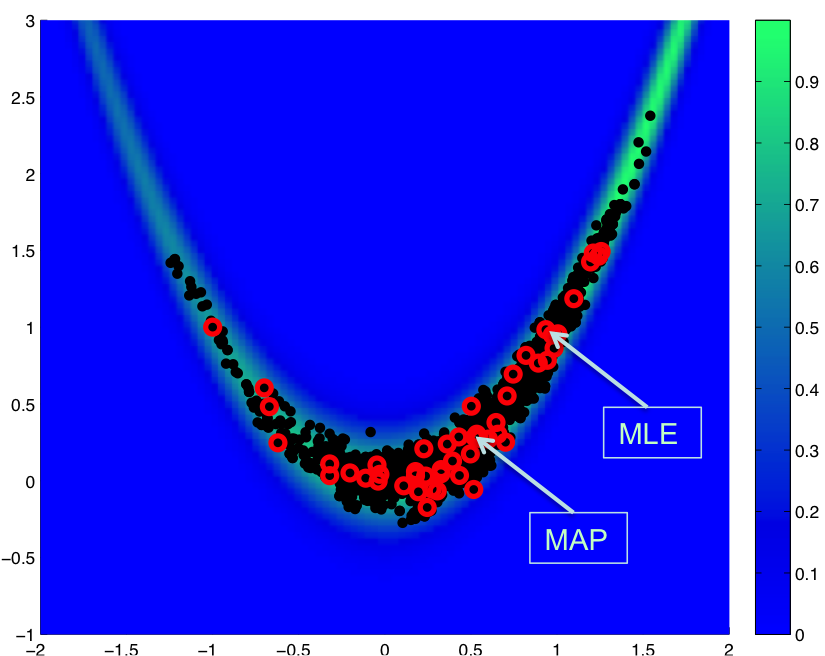
\includegraphics{images/rosen_restart_mle_map}}
  \subfigure[Rejection rates.]{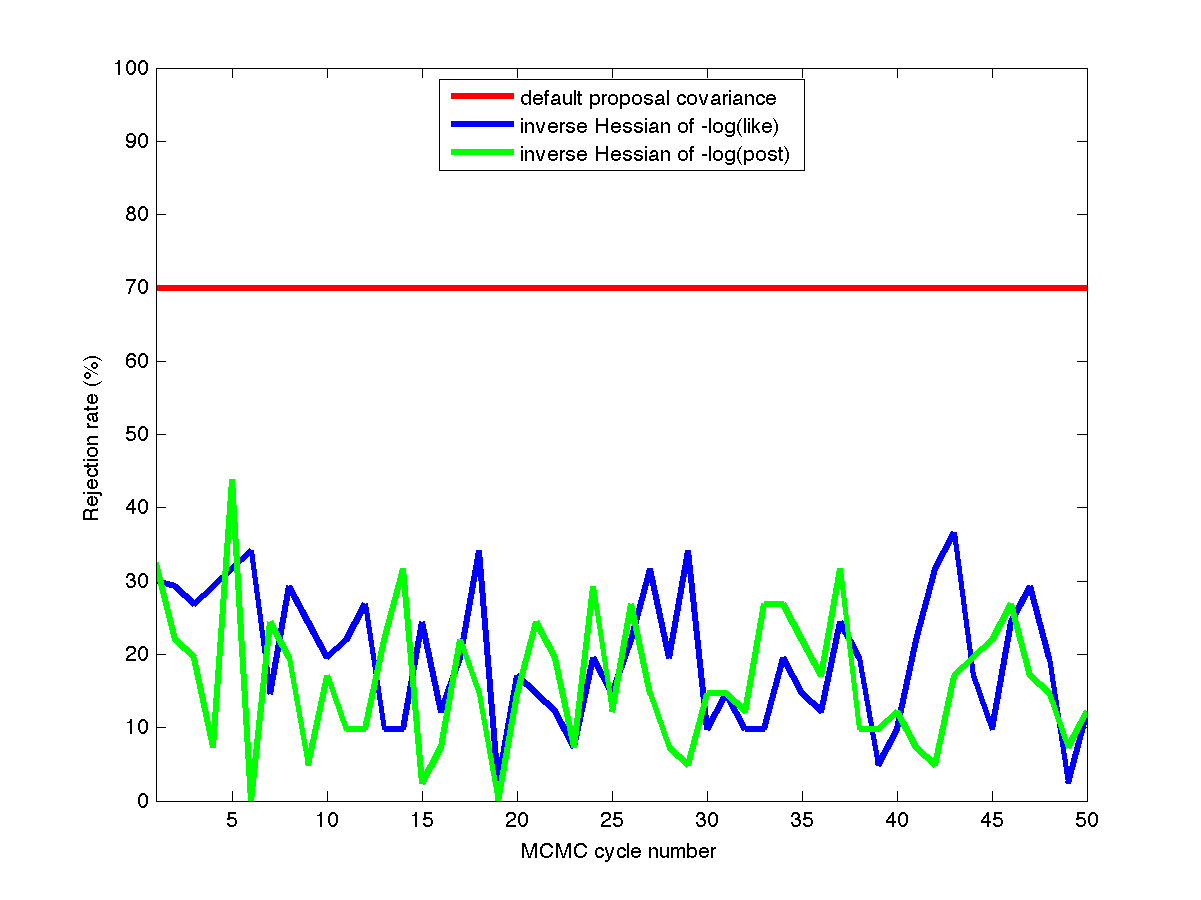
\includegraphics{images/rosen_pce_m11_50up_stdnormal_rejection}}
  \end{subfigmatrix}
  \caption{MCMC with Hessian-based proposals and standard normal prior. Left shows chain with 2000 total samples (black points) and 50 proposal updates (red circles) using the inverse of the misfit Hessian. Right shows rejection rates for misfit Hessian-based and posterior Hessian-based proposals compared to default prior covariance proposal.}
\label{fig:rosen_restart}
\end{figure}
A standard normal prior is not a strong prior in this case, and
the posterior is likelihood dominated.  This leads to similar
performance from misfit Hessian-based proposals and posterior
Hessian-based proposals, with average rejection rates of 70\%, 19.5\%,
and 16.4\% for prior-based, misfit Hessian-based, and posterior
Hessian-based cases, respectively.
